\documentclass[main.tex]{subfiles}
\begin{document}

For test generation, the ModelTestRelax(MTR) framework \cite{mtr} was used with different parameters.

\subsection{Random walk - 100\% transition coverage}
\begin{figure}[H]
    \centering
    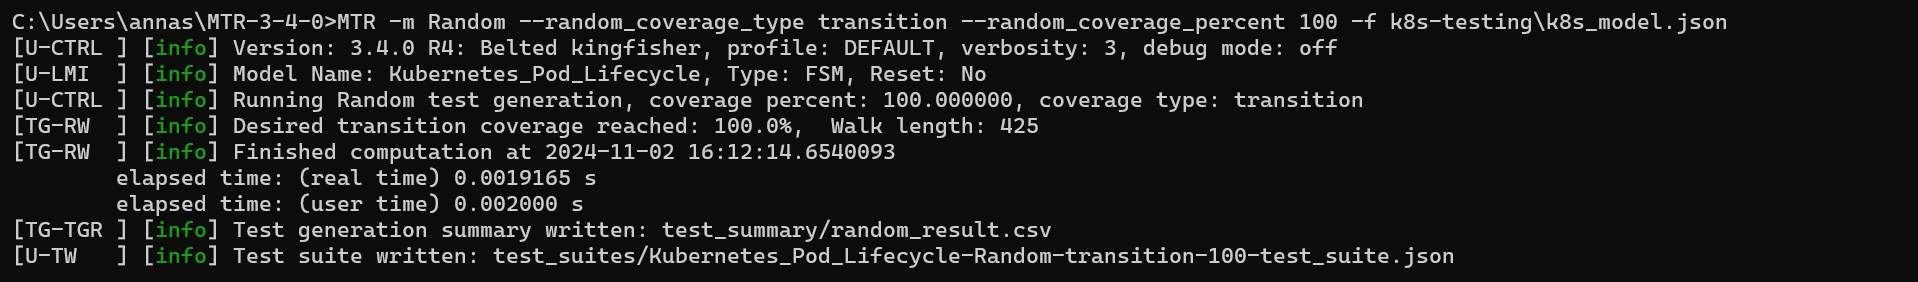
\includegraphics[width=\textwidth]{test_results/random_100coverage.png}
    \caption{Random walk - 100\% transition coverage}
    \label{fig:random_100}
\end{figure}


\subsection{Random walk - 75\% transition coverage}
\begin{figure}[H]
    \centering
    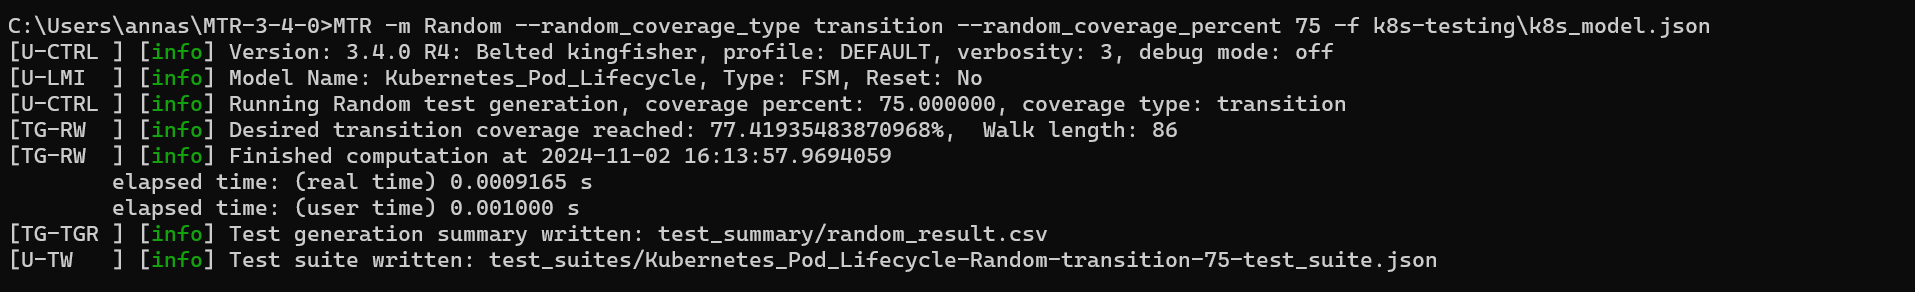
\includegraphics[width=\textwidth]{test_results/random_75coverage.png}
    \caption{Random walk - 75\% transition coverage}
    \label{fig:random_75}
\end{figure}


\subsection{All-state}
\begin{figure}[H]
    \centering
    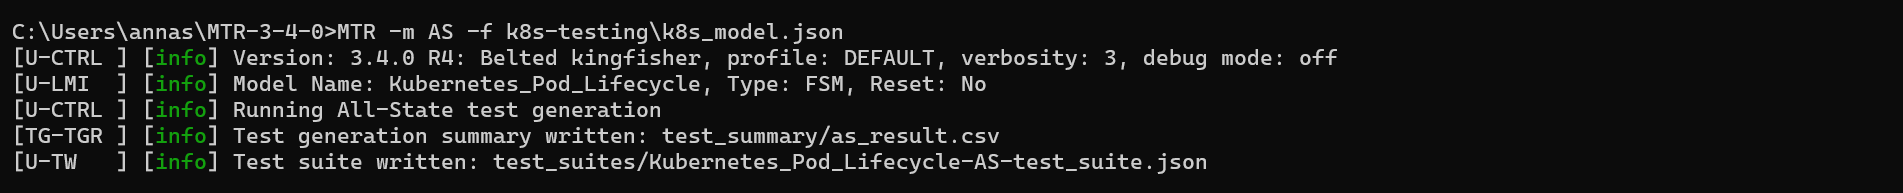
\includegraphics[width=\textwidth]{test_results/all_state.png}
    \caption{All-state}
    \label{fig:all_state}
\end{figure}


\subsection{Transition tour}
\begin{figure}[H]
    \centering
    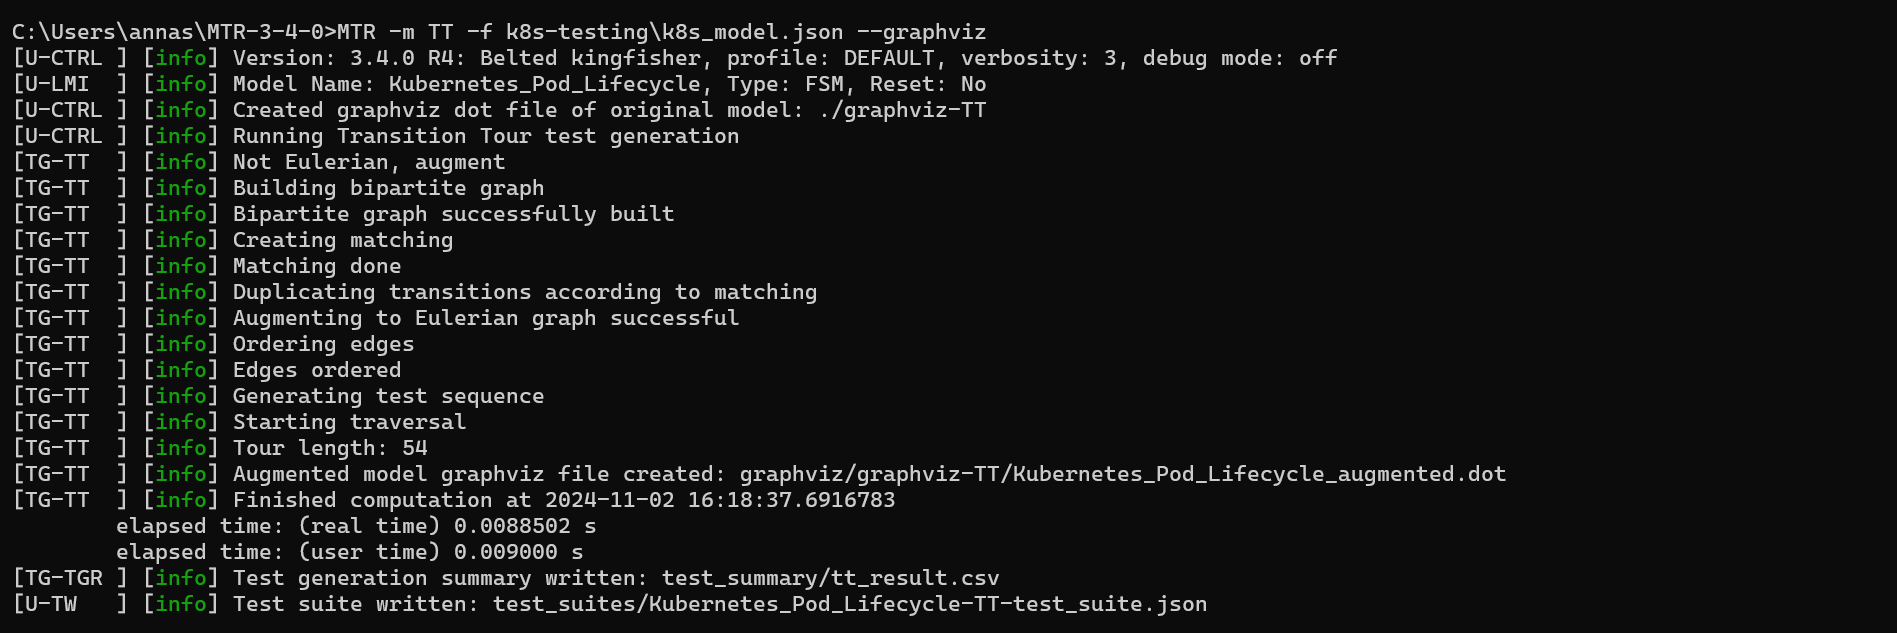
\includegraphics[width=\textwidth]{test_results/transition_tour_graphviz.png}
    \caption{Transition tour}
    \label{fig:transition_tour}
\end{figure}

This is the Graphviz output:
\begin{figure}[H]
    \centering
    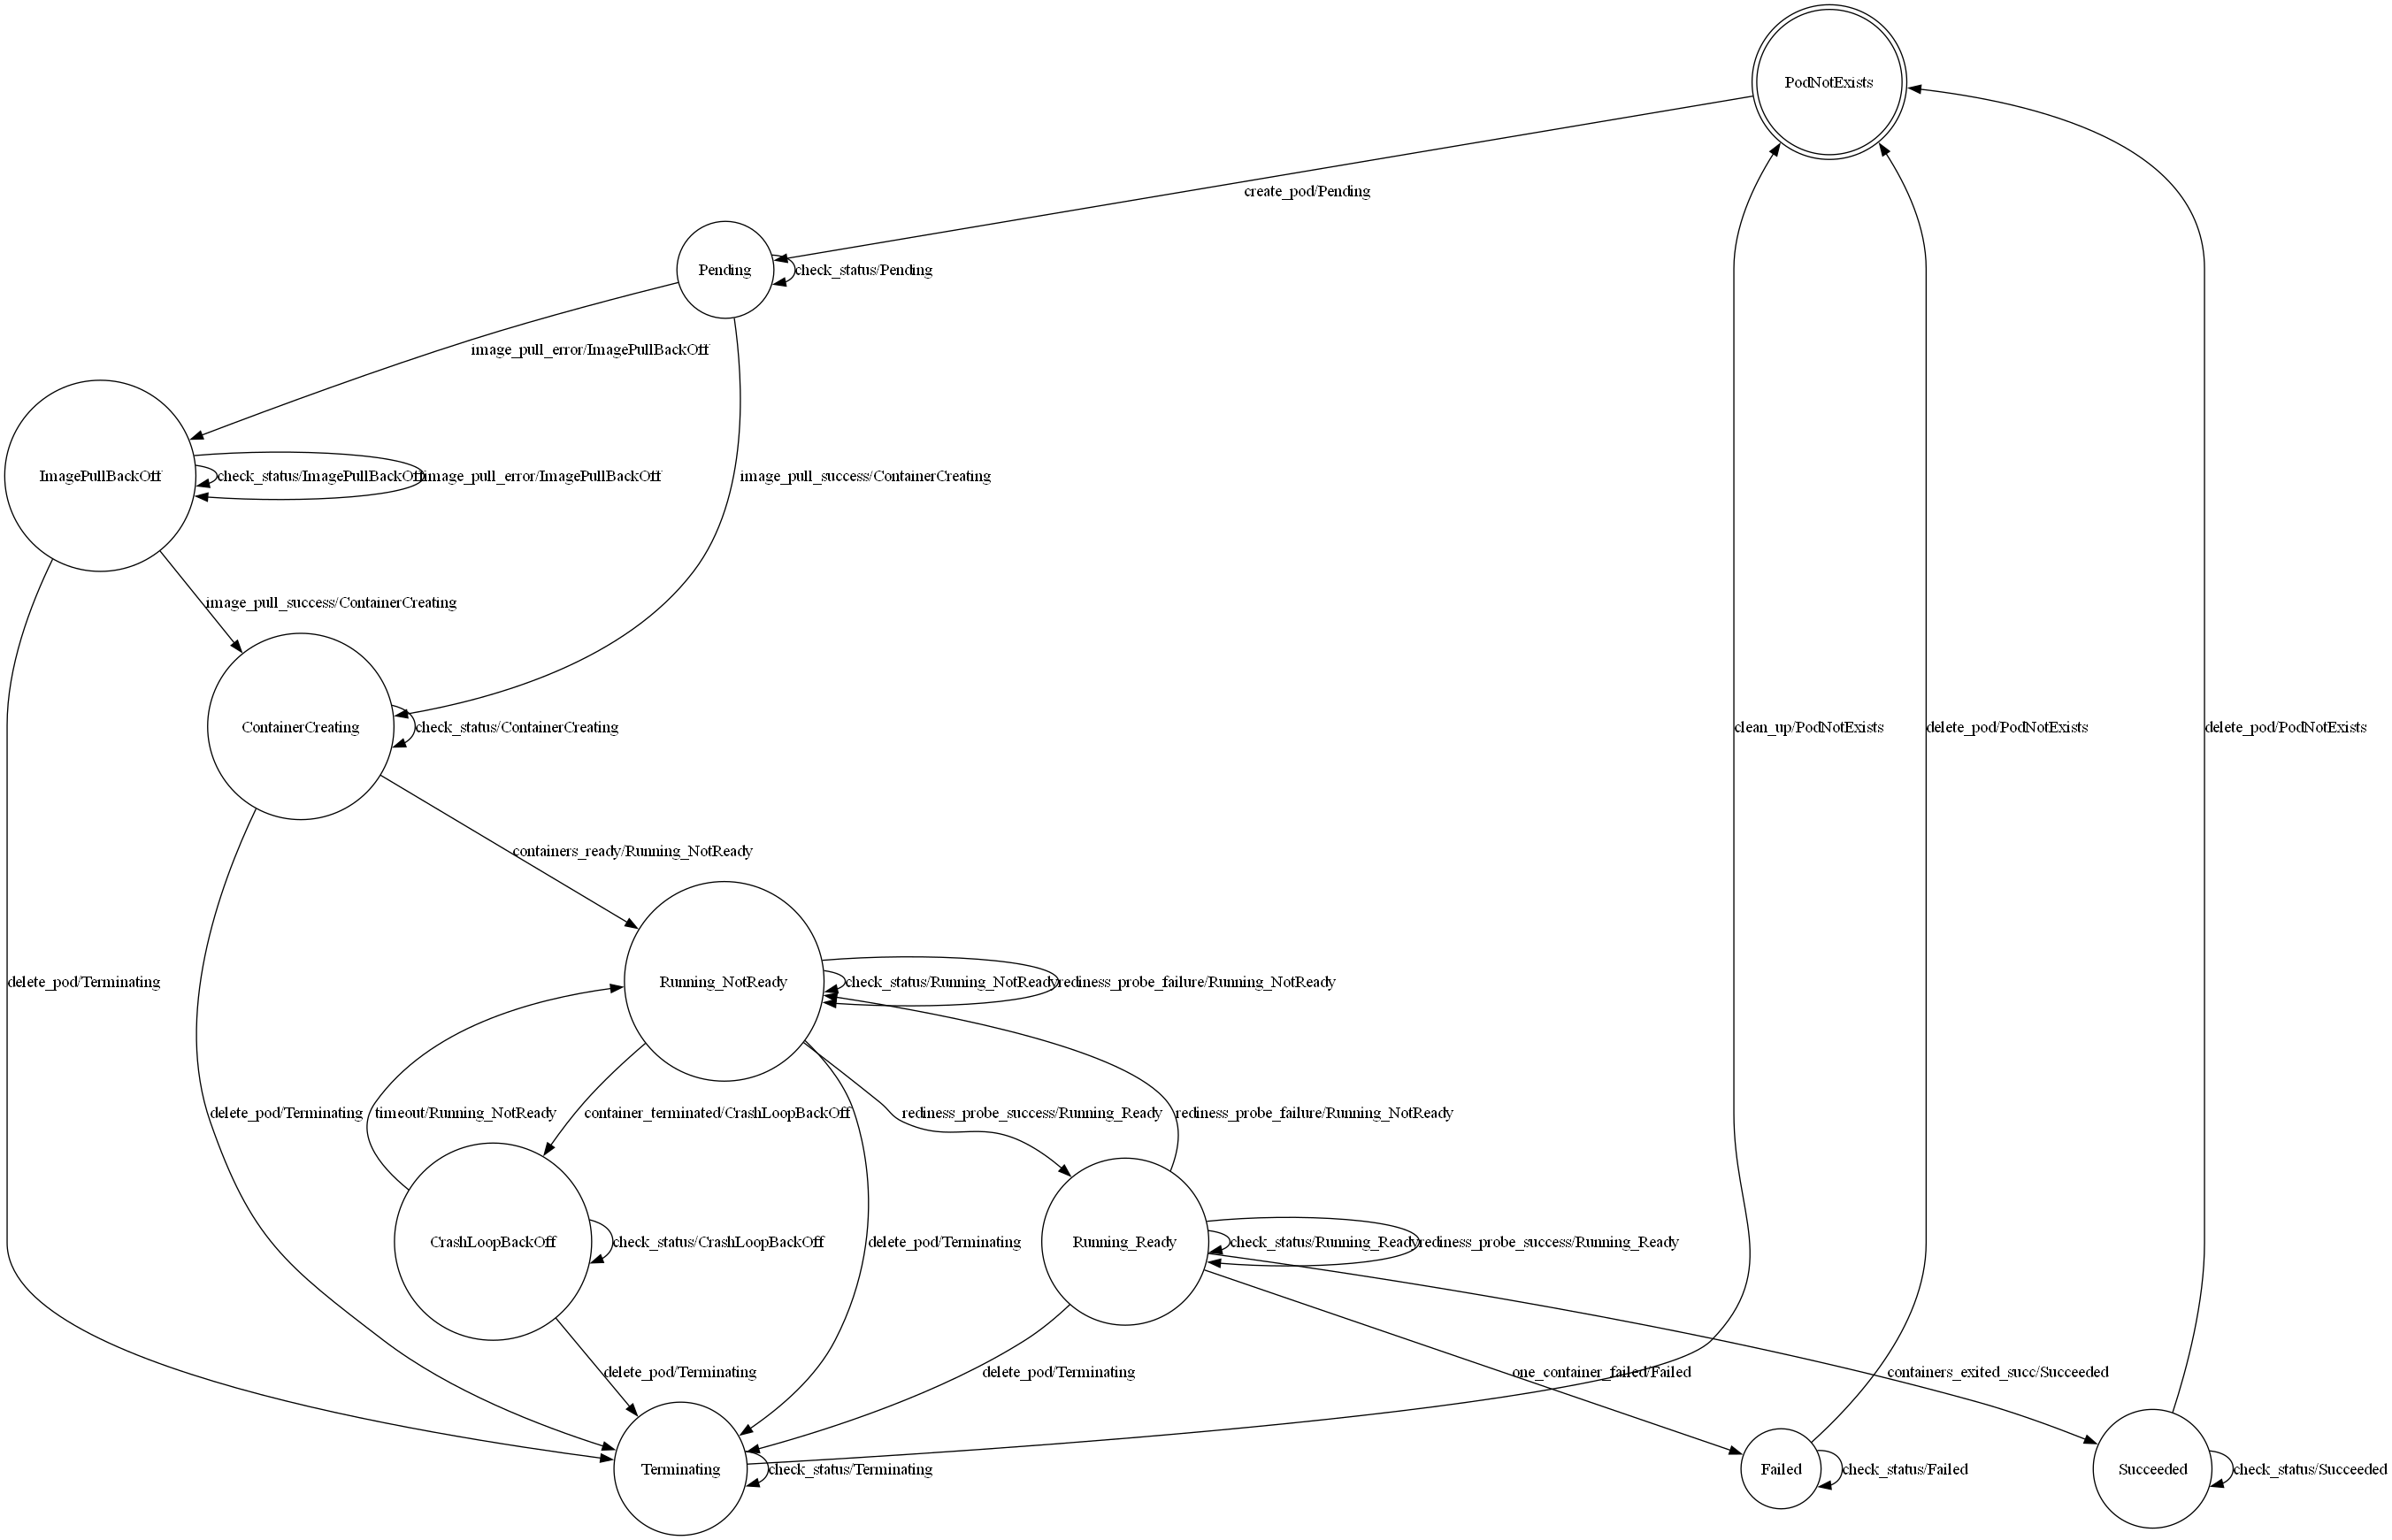
\includegraphics[width=\textwidth]{test_results/tt_image.png}
    \caption{Grapviz result}
    \label{fig:grapviz}

\end{figure}


The generated test suites and result can be found in the github repository: \url{https://github.com/annasz11/kubernetes-mbt}.

\end{document}